% !TEX program = xelatex
% 机器学习课程分组演讲（5 分钟陈述）—— 基于机器学习的台风分类与路径预测
% 编译方式：xelatex 演讲PPT.tex（连续编译两次以更新顶部导航与页码）
\documentclass{beamer}
\usepackage[fontset=mac]{ctex}
\usepackage{hyperref}
\usepackage[T1]{fontenc}

% other packages
\usepackage{latexsym,amsmath,xcolor,multicol,booktabs}
\usepackage{graphicx,listings,stackengine}
\usepackage{tikz}
\usetikzlibrary{positioning,arrows.meta}
\providecommand{\calligra}{\itshape}

\author[徐诗霖\ 蔡奕锴\ 李炜焜]{徐诗霖\and 蔡奕锴\and 李炜焜}
\title[基于机器学习的台风分类、路径预测与登录衰减]{基于机器学习的台风分类、路径预测与登录衰减}
\subtitle{机器学习课程分组演讲}
\institute[计算机科学与工程学院]{计算机科学与工程学院}
\date{2026 年 10 月}
\usepackage{UESTC}

% 覆盖模板默认的“逐节目录页”，为 5 分钟陈述节省页数
\AtBeginSection[]{}
\AtBeginSubsection[]{}
\setbeamertemplate{navigation symbols}{}

% 主讲人标注（评分要求：在 PPT 中标注主讲人）
\newcommand{\speaker}[1]{\hfill{\normalfont\scriptsize\kaishu\color{uestc!30!white}主讲\,#1}}

% defs
\definecolor{deepblue}{rgb}{0,0,0.5}
\definecolor{deepred}{rgb}{0.6,0,0}
\definecolor{deepgreen}{rgb}{0,0.5,0}
\definecolor{halfgray}{gray}{0.55}

\lstset{
    basicstyle=\ttfamily\scriptsize,
    keywordstyle=\bfseries\color{deepblue},
    commentstyle=\color{deepgreen},
    stringstyle=\color{deepgreen},
    showstringspaces=false,
    numbers=none,
    frame=single,
    rulecolor=\color{uestc!40},
    breaklines=true,
    columns=fullflexible,
}

\begin{document}

\kaishu
\begin{frame}
    \titlepage
    \begin{figure}[htpb]
        \begin{center}
            
\includegraphics[width=0.13\linewidth]{pic/logo.pdf}
        \end{center}
    \end{figure}
\end{frame}

% ==================== 报告提纲 ====================
\begin{frame}{报告提纲\speaker{徐诗霖}}
    \small
    \begin{enumerate}
        \item \textbf{问题定义} —— 研究背景 · 三个核心子问题
              
        \item \textbf{技术方案} —— 数据工程 · 分类 / 路径预测 / 登陆衰减建模
              
        \item \textbf{实验结果} —— 台风“贝碧嘉”案例验证
              
        \item \textbf{结论与展望} —— 技术亮点 · 不足与改进
              
    \end{enumerate}
    \vfill
    
\end{frame}

% ==================== 问题定义 ====================
\section{问题定义}

\begin{frame}{研究背景：台风预测为何是机器学习问题\speaker{徐诗霖}}
    \begin{columns}
        \begin{column}{0.52\textwidth}
            \textbf{现实需求}
            \begin{itemize}
                \item 台风突发性强、破坏力大，狂风、暴雨、风暴潮并发
                \item 准确预测可延长预警提前量，支撑人员疏散与应急资源调配
            \end{itemize}
            \vspace{0.4em}
            \textbf{预测难点}
            \begin{itemize}
                \item 内力（地转偏向力）与外力（副热带高压）耦合作用
                \item 路径与影响因素高度非线性，存在打转、停滞现象
            \end{itemize}
        \end{column}
        \begin{column}{0.44\textwidth}
            \begin{block}{机器学习视角}
                台风路径预测本质上是一个\textbf{时空序列预测问题}：
                \begin{itemize}
                    \item \textbf{时序依赖}：台风自身历史运动状态
                    \item \textbf{空间融合}：气压、风场、海温等环境因素
                    \item \textbf{数据基础}：1945--2023 年近 80 年观测
                \end{itemize}
            \end{block}
        \end{column}
    \end{columns}
\end{frame}

\begin{frame}{问题定义：三个核心子问题\speaker{徐诗霖}}
    \centering
    \footnotesize
    \renewcommand{\arraystretch}{1.5}
    \begin{tabular}{p{0.14\textwidth}p{0.34\textwidth}p{0.19\textwidth}p{0.16\textwidth}}
        \toprule
        \textbf{子问题} & \textbf{任务（输入 $\to$ 输出）} & \textbf{验证案例} & \textbf{评价指标} \\
        \midrule
        问题一\newline 台风分类 &
        强度、风速、气压等特征 $\to$ 类别；区分\textbf{夏季 / 秋季台风} &
        2024 年 7 月、9 月台风 &
        准确率、混淆矩阵 \\
        问题二\newline 路径预测 &
        历史运动状态 + 环境因素 $\to$ 未来 \textbf{6 / 12 / 24 h} 中心位置 &
        “贝碧嘉” 9.13--17 &
        大圆距离、RMSE、DTW \\
        问题三\newline 登陆衰减 &
        风速 $V \to$ 降水 $P$；距中心距离 $d \to$ 降水 $P$ &
        “贝碧嘉” 9.16--18 &
        RMSE、$R^2$、残差分析 \\
        \bottomrule
    \end{tabular}

    \vspace{0.6em}
    \begin{block}{问题的统一抽象}\small
        三者共享同一套数据管线与评估思想：均为\textbf{从历史观测中学习非线性映射}，差异仅在映射的目标空间。
    \end{block}
\end{frame}

% ==================== 技术方案 ====================
\section{技术方案}

\begin{frame}{技术路线总览\speaker{徐诗霖}}
    \centering
    \resizebox{0.96\textwidth}{!}{%
    \begin{tikzpicture}[
        font=\scriptsize,
        box/.style={draw=uestc, thick, rounded corners=3pt, fill=uestc!8,
                    align=center, inner sep=4pt, minimum height=2.4em},
        arr/.style={-{Stealth[length=5pt]}, thick, draw=uestc!80}]
        \node[box] (data) at (0,2.0) {\textbf{数据}\\[-1pt] 1945--2023 台风路径集合\\[-1pt] + 2024 年个例观测};
        \node[box] (prep) at (4.6,2.0) {\textbf{数据工程}\\[-1pt] 插值 · 去异常 · 标准化 · PCA};
        \node[box] (m1) at (0,0) {\textbf{问题一：分类}\\[-1pt] K-Means + 决策树 / SVM / LSTM};
        \node[box] (m2) at (5.1,0) {\textbf{问题二：路径预测}\\[-1pt] SVR $\to$ LSTM $\to$ CNN-LSTM+注意力};
        \node[box] (m3) at (10.0,0) {\textbf{问题三：登陆衰减}\\[-1pt] 幂律 / 指数 / 高斯 + RF / GPR};
        \node[box] (eval) at (4.9,-2.0) {\textbf{评估}\\[-1pt] 混淆矩阵 · RMSE · DTW · 残差分析};
        \draw[arr] (data) -- (prep);
        \draw[arr] (prep.south) -- (m1.north);
        \draw[arr] (prep.south) -- (m2.north);
        \draw[arr] (prep.south) -- (m3.north);
        \draw[arr] (m1.south) -- (eval.west);
        \draw[arr] (m2.south) -- (eval.north);
        \draw[arr] (m3.south) -- (eval.east);
    \end{tikzpicture}}

    \vspace{0.4em}
    \begin{itemize}\small
        \item 技术主线：\textbf{历史序列建模、环境特征融合、直接预测位移、独立事件验证}
        \item 三个子问题共享数据管线，评估口径按任务分别设定
    \end{itemize}
\end{frame}

\begin{frame}{数据工程与特征分析\speaker{徐诗霖}}
    \begin{columns}
        \begin{column}{0.50\textwidth}
            \begin{enumerate}\small
                \item \textbf{缺失填补}：拉格朗日插值（移动方向、速度）
                \item \textbf{异常检测}：箱线法剔除野值（风速 $>110$ m/s 等）
                \item \textbf{标准化}：$Z=(X-\mu)/\sigma$，参数\textbf{仅由训练集估计}
                \item \textbf{降维}：PCA，累计贡献率 $>85\%$
            \end{enumerate}
            \vspace{0.2em}
            {\footnotesize\textcolor{uestc}{\textbf{数据划分}}\ 按年份与\textbf{完整台风事件}划分训练 / 验证 / 测试集，同一台风不跨集合，杜绝信息泄漏。}
        \end{column}
        \begin{column}{0.46\textwidth}
            \centering
            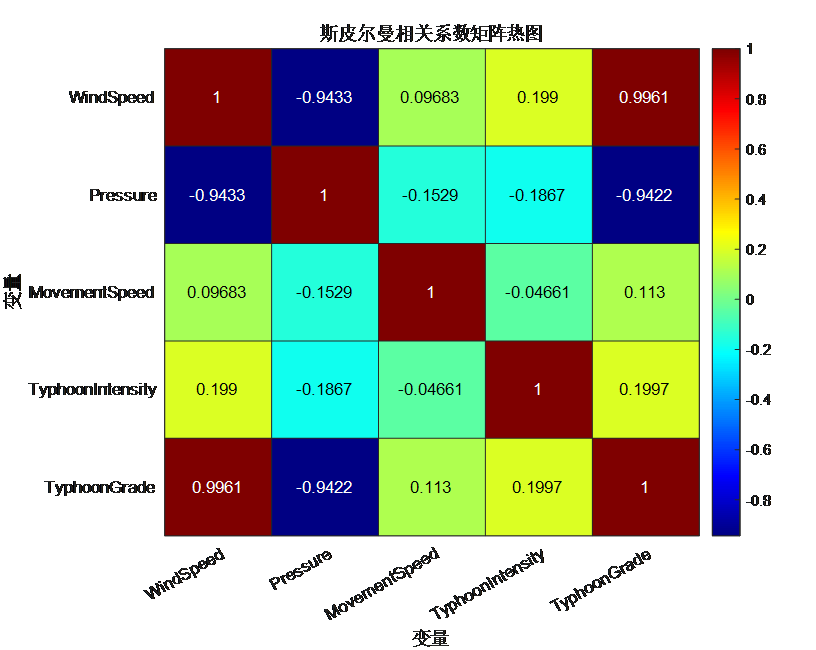
\includegraphics[width=1.2\linewidth]{figures/热力图.png}

            {\footnotesize 斯皮尔曼相关系数矩阵}
        \end{column}
    \end{columns}
    \begin{block}{特征分析的独立判断}\footnotesize
        风速--等级 $r=0.996$、风速--气压 $r=-0.943$：强相关提示\textbf{特征冗余}，为特征筛选与模型输入设计提供量化依据，而非全量喂入模型。
    \end{block}
\end{frame}

\begin{frame}{问题一：台风分类模型\speaker{蔡奕锴}}
    \begin{columns}
        \begin{column}{0.42\textwidth}
            \centering
            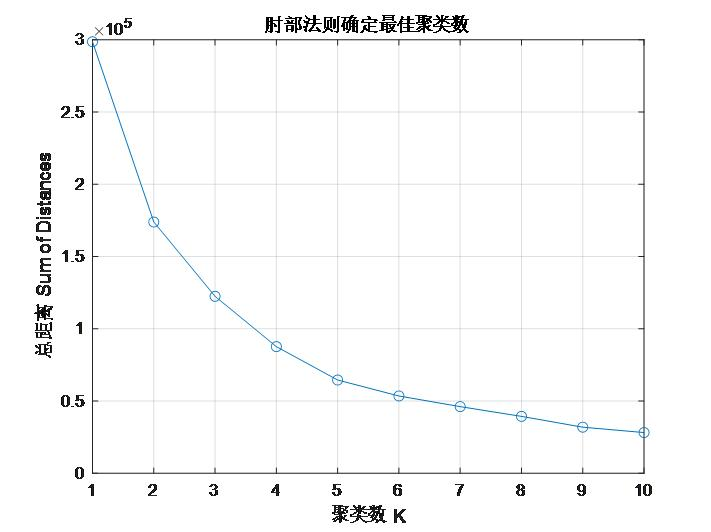
\includegraphics[width=0.86\linewidth]{figures/肘部法.jpg}

            {\footnotesize 肘部法则确定聚类数 $K=3$}\\[3pt]
            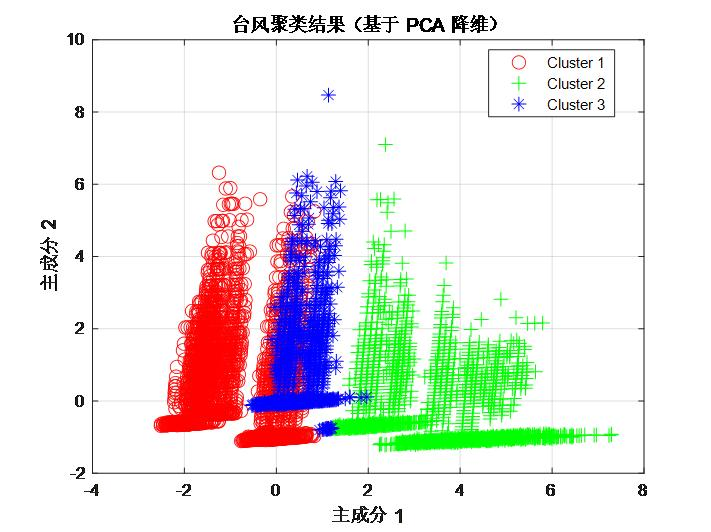
\includegraphics[width=0.86\linewidth]{figures/台风聚类的结果.jpg}

            {\footnotesize PCA 降维后的聚类结构}
        \end{column}
        \begin{column}{0.54\textwidth}
            \textbf{两阶段方法}
            \begin{itemize}
                \item \textbf{无监督探索}：K-Means 聚类观察特征空间的自然结构
                \item \textbf{监督建模}：决策树 $\to$ SVM $\to$ LSTM，交叉验证比较精度
            \end{itemize}
            \vspace{0.4em}
            \begin{block}{结论：夏 / 秋台风差异}
                \begin{itemize}\small
                    \item 夏台风（6--8 月）：数量多、风速高，多向西北移动
                    \item 秋台风（9--11 月）：生成纬度更高，平均强度不弱、路径更多变
                    \item 2024 年 7 月 / 9 月个例的判别结果与气象事实一致
                \end{itemize}
            \end{block}
        \end{column}
    \end{columns}
\end{frame}

\begin{frame}{问题二：递进式路径预测模型\speaker{蔡奕锴}}
    \centering\small
    外推基线 $\to$ SVR $\to$ LSTM $\to$ CNN-LSTM $\to$ \textbf{+通道注意力}\\[1pt]
    {\footnotesize\color{halfgray} 每一层针对上一层的明确缺陷：无法响应环境变化 $\to$ 忽略时序依赖 $\to$ 缺空间特征 $\to$ 特征无差异加权}

    \vspace{0.4em}
    \begin{itemize}\small
        \item \textbf{LSTM}：三门控机制（遗忘 / 输入 / 输出）建模过去 24 h 状态序列的长程依赖
        \item \textbf{CNN--LSTM 双分支}：CNN 提取环境场空间特征，LSTM 提取时序特征，经\textbf{通道注意力}自适应加权融合
    \end{itemize}
    \begin{center}
        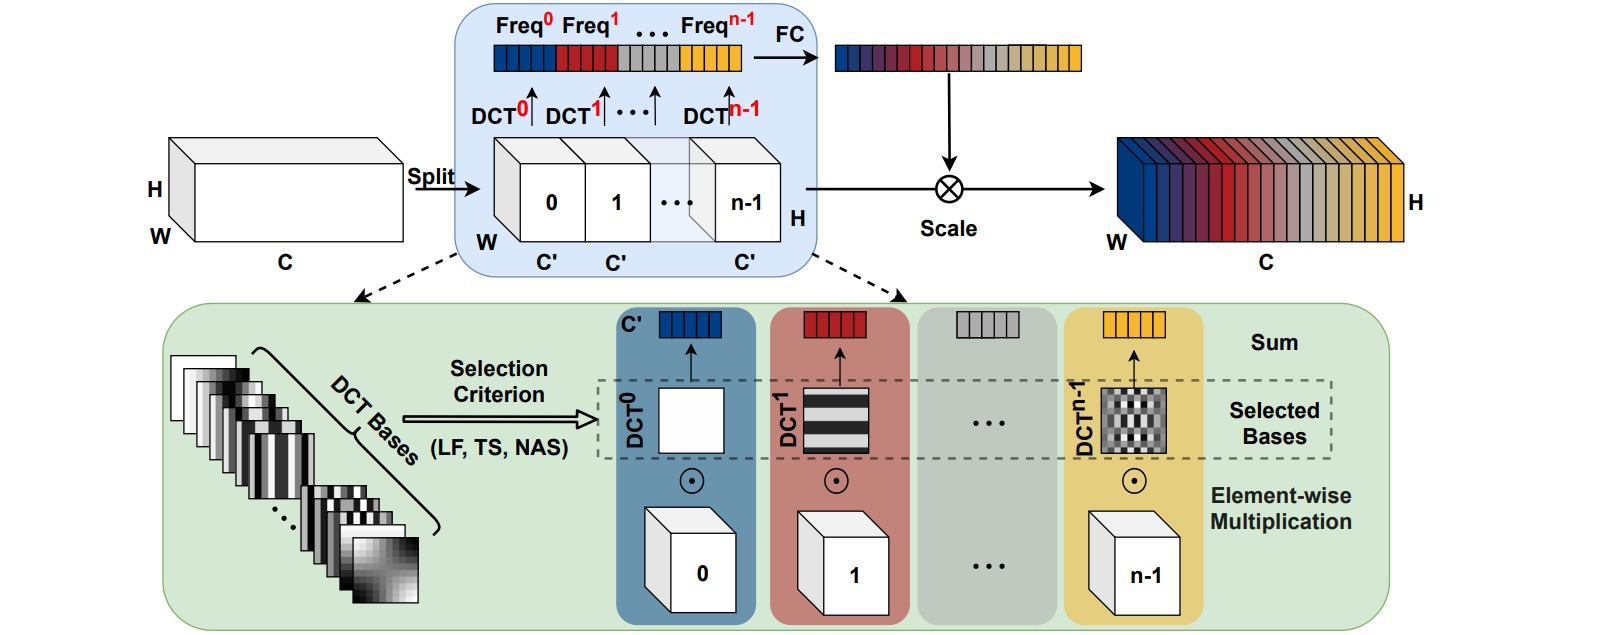
\includegraphics[width=0.60\linewidth]{figures/神经网络通道图.jpg}
    \end{center}
    {\footnotesize\color{halfgray} 通道注意力：压缩（Squeeze）全局信息 $\to$ 激励（Excitation）生成通道权重，突出关键特征通道}
\end{frame}

\begin{frame}[fragile]{问题二：关键设计与实验规范\speaker{蔡奕锴}}
    \begin{columns}
        \begin{column}{0.54\textwidth}
\begin{lstlisting}
# 目标重参数化：预测位移而非速度
delta = pos[t + h] - pos[t]   # h = 6/12/24 h
X = feats[t-24:t]             # 过去 24 h 状态序列
y_hat = CNN_LSTM_SE(X)        # 时空 + 通道注意力
loss = mse_loss(y_hat, delta)

# 防信息泄漏：按完整台风事件划分
train, test = split_by_storm_id(...)
\end{lstlisting}
        \end{column}
        \begin{column}{0.42\textwidth}
            \begin{itemize}\small
                \item \textbf{防信息泄漏}：标准化参数仅由训练集估计；同一台风的相邻样本不跨集合
                \item \textbf{消融实验}：逐一移除 CNN 分支 / 注意力模块，量化各模块贡献
                \item \textbf{困难样本}：单独分析转向、登陆、快速移动样本
            \end{itemize}
        \end{column}
    \end{columns}
    \begin{block}{为什么直接预测未来位移？}\footnotesize
        以“移动速度”为输出时，位置需经积分还原，误差随步长累积且起点不定；位移目标与“预测未来位置”任务\textbf{直接对齐}，逐段累加即可还原完整路径。
    \end{block}
\end{frame}

\begin{frame}{路径预测结果：台风“贝碧嘉”（9 月 13--17 日每日 14 时）\speaker{蔡奕锴}}
    \begin{columns}
        \begin{column}{0.50\textwidth}
            \centering
            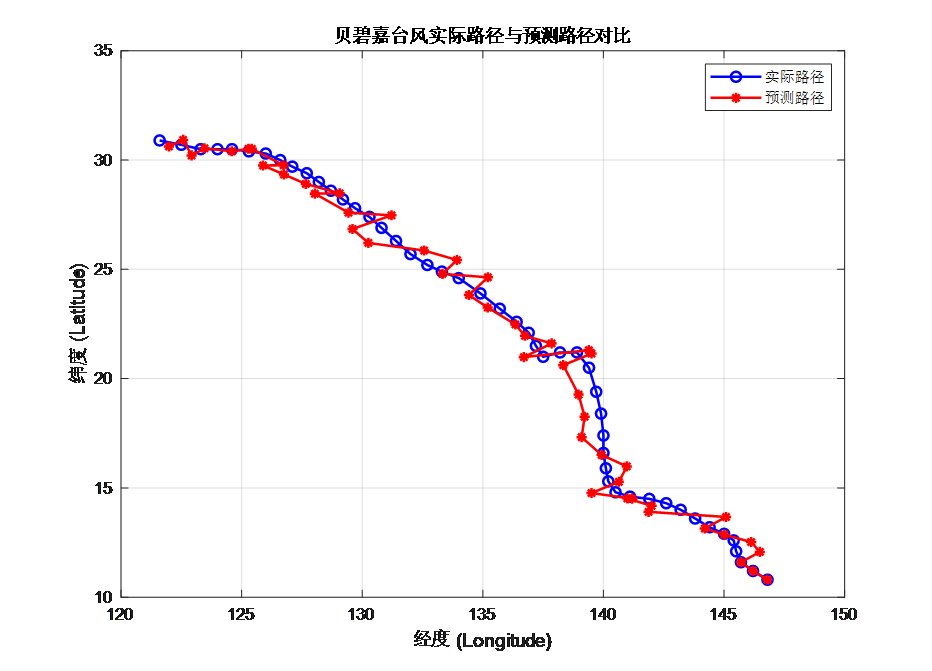
\includegraphics[width=\linewidth]{figures/路径对比图.png}

            {\footnotesize 预测路径与实际路径对比}
        \end{column}
        \begin{column}{0.46\textwidth}
            \begin{block}{定量指标}\small
                RMSE $= 0.232$\qquad DTW 距离 $= 94.25$
            \end{block}
            \begin{block}{定性分析}\small
                \begin{itemize}
                    \item 大方向与整体趋势准确，平稳段高度重合
                    \item 急转弯处预测\textbf{滞后}：时序依赖未完全捕捉
                    \item 训练 / 验证 / 测试损失接近，无明显过拟合
                \end{itemize}
            \end{block}
        \end{column}
    \end{columns}
\end{frame}

\begin{frame}{问题三：登陆后风速与降水衰减建模\speaker{李炜焜}}
    \begin{columns}
        \begin{column}{0.50\textwidth}
            \begin{block}{物理先验：风速 -- 降水关系}\small
                动力学：强风增强对流、促进水汽上升；热力学：强风加剧海面蒸发
                \begin{itemize}
                    \item 幂律模型：$P = aV^b$
                    \item 指数模型：$P = ae^{bV}$
                    \item 多项式：$P = c_0 + c_1V + \cdots + c_nV^n$
                \end{itemize}
            \end{block}
            \begin{block}{空间衰减：降水 -- 距离关系}\small
                \begin{itemize}
                    \item 指数衰减：$P = P_0e^{-\lambda d}$
                    \item 高斯分布：$P = P_0\,e^{-\frac{(d-\mu)^2}{2\sigma^2}}$
                \end{itemize}
            \end{block}
        \end{column}
        \begin{column}{0.46\textwidth}
            \begin{block}{多变量数据驱动扩展}\small
                引入\textbf{方位角、湿度、风切变、地形}等协变量，采用\textbf{随机森林}、\textbf{高斯过程回归}刻画降水分布的空间不对称性
            \end{block}
            \begin{itemize}\small
                \item 多模型竞争拟合 + \textbf{残差分析}择优
                \item 体现“物理先验 + 数据驱动”的互补建模思想
            \end{itemize}
        \end{column}
    \end{columns}
\end{frame}

\begin{frame}{降水建模结果：台风“贝碧嘉”登陆后（9 月 16--18 日）\speaker{李炜焜}}
    \begin{columns}
        \begin{column}{0.48\textwidth}
            \centering
            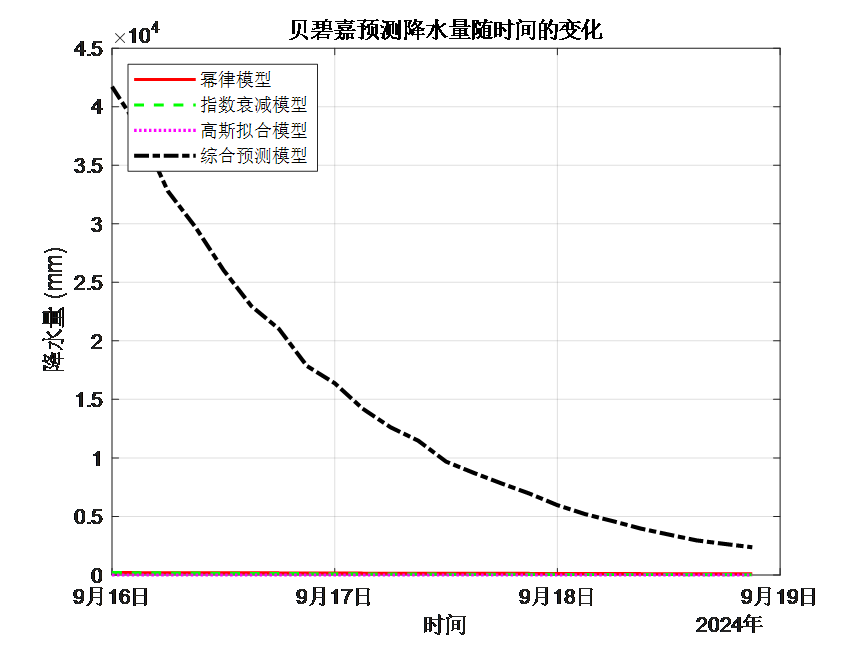
\includegraphics[width=0.92\linewidth]{figures/贝碧嘉台风预测降水量变化.png}

            {\footnotesize 综合预测模型捕捉登陆后降水衰减趋势}
        \end{column}
        \begin{column}{0.48\textwidth}
            \centering
            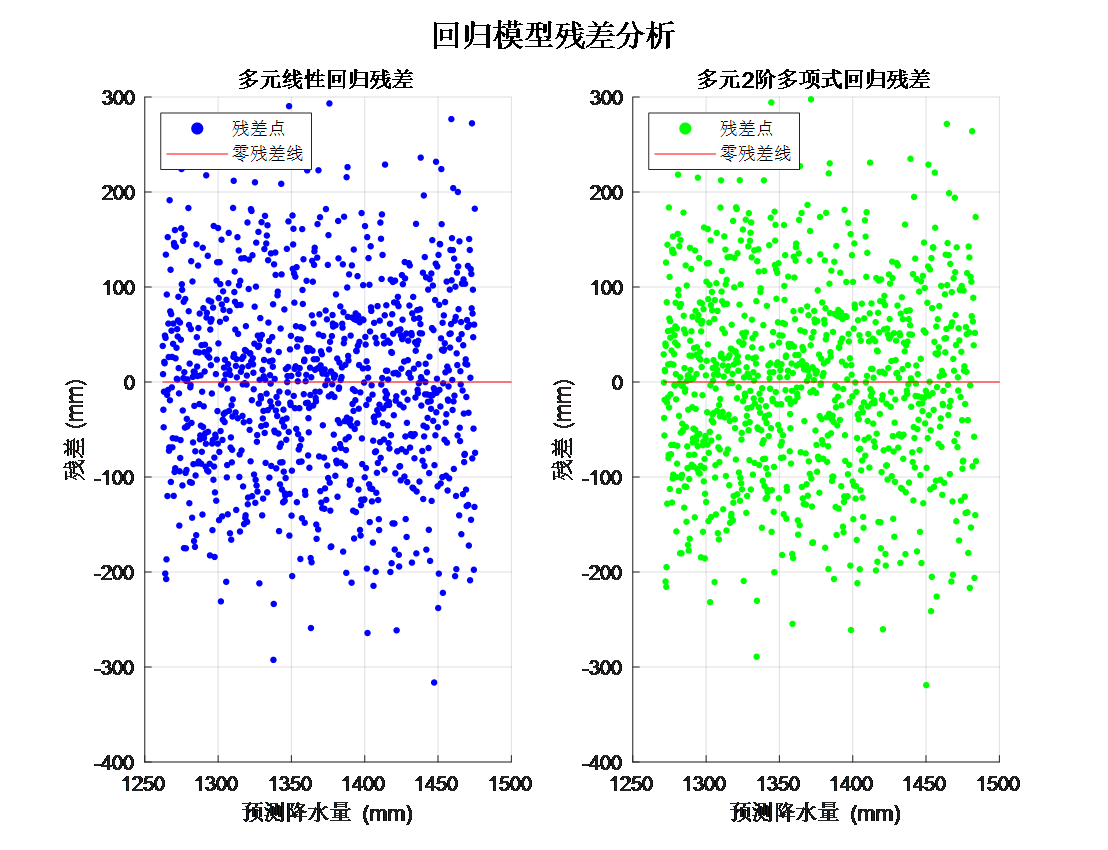
\includegraphics[width=0.98\linewidth]{figures/模型预测降水量与实际降水量的比较.png}

            {\footnotesize 残差围绕零线分布、无系统性偏差}
        \end{column}
    \end{columns}
    \vspace{0.4em}
    \begin{block}{结论}\small
        综合预测模型\textbf{显著优于单一拟合}；风速与降水正相关，降水量在台风中心附近达到峰值、随距离呈指数衰减。
    \end{block}
\end{frame}

% ==================== 结论 ====================
\section{结论}

\begin{frame}{结论：技术亮点与展望\speaker{李炜焜}}
    \begin{block}{技术亮点}
        \begin{enumerate}\small
            \item \textbf{严格数据治理}：标准化仅用训练集、按完整台风事件划分——从源头杜绝信息泄漏
            \item \textbf{递进式基线 + 消融实验}：每一层模型的引入都有明确动机与可量化贡献
            \item \textbf{目标重参数化}：直接预测未来位移，预测目标与任务对齐
            \item \textbf{物理先验 + 数据驱动}：幂律 / 指数 / 高斯约束结合随机森林 / 高斯过程回归
        \end{enumerate}
    \end{block}
    \begin{columns}
        \begin{column}{0.50\textwidth}
            \textbf{不足}
            \begin{itemize}\small
                \item 环境场数据（ERA5 风场、位势高度场）尚未融合
                \item 转向拐点预测存在滞后
            \end{itemize}
        \end{column}
        \begin{column}{0.46\textwidth}
            \textbf{展望}
            \begin{itemize}\small
                \item 集成学习降低预测方差
                \item 物理约束神经网络（PINN）注入动力学先验
            \end{itemize}
        \end{column}
    \end{columns}
    \vspace{0.3em}
    {\scriptsize\color{halfgray} 主要参考：Gao et al. (2018) LSTM 路径预报 · Giffard-Roisin et al. (2020) 环境场融合位移预测 · Liu et al. (2022) DBF-Net · He et al. (2023) 双注意力 ConvLSTM}
\end{frame}

\begin{frame}
    \begin{center}
        {\Huge\calligra 谢谢！}\\[1.2em]
        \large 恳请各位老师、同学批评指正\\[1em]
        \normalsize
        主讲分工：徐诗霖（PPT 制作 · 研究背景 · 技术路线）\quad 蔡奕锴（台风分类 · 路径预测）\quad 李炜焜（衰减建模 · 结论）\\[0.6em]
        \footnotesize
        计算机科学与工程学院 \quad 2026 年 10 月
    \end{center}
\end{frame}

\end{document}
